\documentclass[boxes, qed]{homework}
\usepackage{xcolor,amsmath,listings}
\usepackage{graphicx}
\graphicspath{ {./images/} }

\name{Rohit Wason}
\course{Math 560}
\term{Spring 2021}
\hwnum{(\#7, Inference of the Mean)}

\newcommand{\bigzero}{\mbox{\normalfont\Large\bfseries 0}}
\newcommand{\rvline}{\hspace*{-\arraycolsep}\vline\hspace*{-\arraycolsep}}

\begin{document}

\begin{problem}Given $\bar{x}=9.289221, s=0.8191156$ and $n=10$
  calculate the $92\%$ two-sided C.I. for $\mu$.
\end{problem}
\begin{solution}\begin{itemize}
  \item $t^*$, a statistic that follows a \textbf{t-distribution}, $t(n-1=7)$ 
  for $C=92\%$, is given by
  \begin{lstlisting}[backgroundcolor = \color{lightgray},language = R]
  qt(0.96,df=7)
  >> 2.046011
  \end{lstlisting}
  \item Hence the $92\%$ confidence interval for $\mu$ is:
    \begin{align*}
      &= \bar{x} \pm t^*\frac{s}{\sqrt{n}}\\
      &= 9.289221 \pm 2.046011 (\frac{0.8191156}{\sqrt{8}})\\
      &= ( 8.696694, 9.881748)
    \end{align*}
\end{itemize}
\end{solution}

\begin{problem}StatsVillage.txt is used.
\end{problem}
\begin{solution}
  (a) The following seed is used
  \begin{lstlisting}[backgroundcolor = \color{lightgray},language = R]
    set.seed(19891)
  \end{lstlisting}

  (b) Here are the summary statistics for two independent SRSs\\

  \begin{tabular}{l|l|l|l|l}
    \hline
    Population & Name & $n$ & $\bar{x}$ & $s$ \\
    \hline
    1 & North & $15$ & $3474.8$ & $7828.715$ \\
    2 & South & $20$ & $7319.15$ & $5318.922$ \\
  \end{tabular}\\

  \begin{enumerate}
    \item Test $H_0:(\mu_1-\mu_2)=0$ vs. $H_a:(\mu_1-\mu_2)<0$
    \item The test statistic: 
      \begin{align*}
        t
        &=
        \frac{(\bar{x_1}-\bar{x_2}) - (\mu_1-\mu_2)}
        {\sqrt{
          \frac{s_1^2}{n_1}
          +\frac{s_2^2}{n_2}
        }}\\
        &=
        \frac{(3474.8-7319.15) - 0}
        {\sqrt{
          \frac{7828.715^2}{15}
          +\frac{5318.922^2}{20}
        }}\\
        &=-1.639167
      \end{align*}
    \item For critical value, $t^*$ first let's calculate degrees of freedom: 
      \begin{align*}
        k
        &=
        \frac{
          (
            \frac{s_1^2}{n_1}
            +\frac{s_2^2}{n_2}
          )^2
        }
        {
          \frac{1}{n_1-1}(\frac{s_1^2}{n_1})^2
          +\frac{1}{n_2-1}(\frac{s_2^2}{n_2})^2
        }\\
        &=
        \frac{
          (
            \frac{7828.715^2}{15}
            +\frac{5318.922^2}{20}
          )^2
        }
        {
          \frac{1}{14}(\frac{7828.715^2}{15})^2
          +\frac{1}{19}(\frac{5318.922^2}{20})^2
        }\\
        &=23.31274\\
        \therefore t^*
        &=t(23.31274)\\
        &\approx 1.714
      \end{align*}
    \item Conclusion: since $|t|=1.639<t^*=1.714$,
      we \textbf{cannot reject the null hypothesis}.
  \end{enumerate}

  (c) The true means: $\mu_1=2838.85 < \mu_2=6982.859$
  which means the population mean of the Southern half \textit{is}
  greater than that of the Northern half.
  The test in (b) rejected the hypothesis that $\mu_2>\mu_1$ and 
  \textbf{did not} detect the difference between them.\\
  I think the other students will reach the same conclusion
  as $n_1,n_2$ are large enough for the samples to follow
  t-distribution.
\end{solution}

\begin{problem}A poll is conducted to gather information about the proportion of voters $p$ who will vote
  for a candidate in a primary election. Assume that the number of voters in the population is very large.
\end{problem}
\begin{solution} (a) $z^*=1.96$ for $95\%$ C.I. 
  For an estimate $p^*$, the margin of error
  \begin{align*}
    1.96\sqrt{\frac{p^*(1-p^*)}{n}} &\le 0.10\\
    3.8416\frac{p^*(1-p^*)}{n} &\le 0.01\\
    n &\ge \frac{3.8416}{0.01} p^*(1-p^*)\\
    &\ge \frac{3.8416}{0.01}(\frac{1}{2})^2
  \end{align*}
  since the above expression maximizes at $p^*=\frac{1}{2}$.\\

  Hence $n\ge96.04$ or $n=97$ is the smallest sample size 
  that will guarantee that the margin of error for this 
  confidence interval will be no more than $0.10$.\\

  (b) The expected \# of successes $n \times p=97 \times 0.20 = 19.4 > 10$\\
  The expected \# of failures = $97 \times 0.80 = 12.8 > 10$. Since both are
  more than $10$, the \textbf{condition to use the large-sample interval is satisfied}.
\end{solution}

\begin{problem}Let $p$ be the probability that the die comes up with the side labeled six. 
  A six-sided die is rolled $100$ times and the side labeled six comes up $27$ times.
  Therefore $\hat{p}=X/n=0.27$.
\end{problem}
\begin{solution}(a) At 99\% confidence interval, $z^*=2.575829$. The CI fpr $p$ is
  \begin{align*}
    &=\hat{p} \pm z^*\sqrt{\frac{\hat{p}(1-\hat{p})}{n}}\\
    &=0.27 \pm 2.575829\sqrt{\frac{0.27(1-0.27)}{100}}\\
    &=(0.1556436,0.3843564)
  \end{align*}

  (b) At $\alpha=0.1$,
  \begin{itemize}
    \item Hypothesis $H_0: p=\frac{1}{6}$ vs. $H_a: p\ne\frac{1}{6}$
    \item Test statistic 
      \begin{align*}
        z^*&=\frac{\hat{p}-p_0}{\sqrt{\frac{p_0(1-p_0)}{n}}}\\
        &=\frac{0.27-0.167}{\sqrt{\frac{0.27(0.73)}{100}}}\\
        &=2.320032
      \end{align*}
    \item $PValue =
      2\times P(z>2.320032) 
      =2\times (1-P(z \le 2.320032))
      =2\times (1-0.9898304)
      =0.02033916
      $
    \item Since $PValue = 0.02033916 < \alpha$ so 
      \textbf{we reject} $H_0: p=\frac{1}{6}$.
  \end{itemize}
\end{solution}

\section{Project details}
\begin{enumerate}
  \item Dataset: I plan to use the  
  \href{https://www.kaggle.com/fedesoriano/stroke-prediction-dataset?select=healthcare-dataset-stroke-data.csv}
  {Stroke Prediction Dataset} that I found on Kaggle for my project. It has $5110$ records. 
  Of of the $12$ variables, some interesting ones are:
  \begin{itemize}
    \item Gender
    \item Ever Married (Yes/No)
    \item Age
    \item Residence Type (Urban/Suburban/Rural)
    \item BMI Level
    \item Had stroke (Yes/No)
  \end{itemize}

  \item We could excplore questions like:
  \begin{itemize}
    \item Effect of BMI on having stroke.
    \item Correlation between Residence Type and BMI.
    \item Whether people in Suburban and Urban setting are more prone to 
    Stroke than those in Rural.
  \end{itemize}

  \item Some summarization:
  \begin{lstlisting}[backgroundcolor = \color{lightgray},language = R]
    mean(stroke$heart_disease)
    [1] 0.05401174
    > mean(stroke$age)
    [1] 43.22661
  \end{lstlisting}

  \item A histogram of ages in the given dataset:\\
  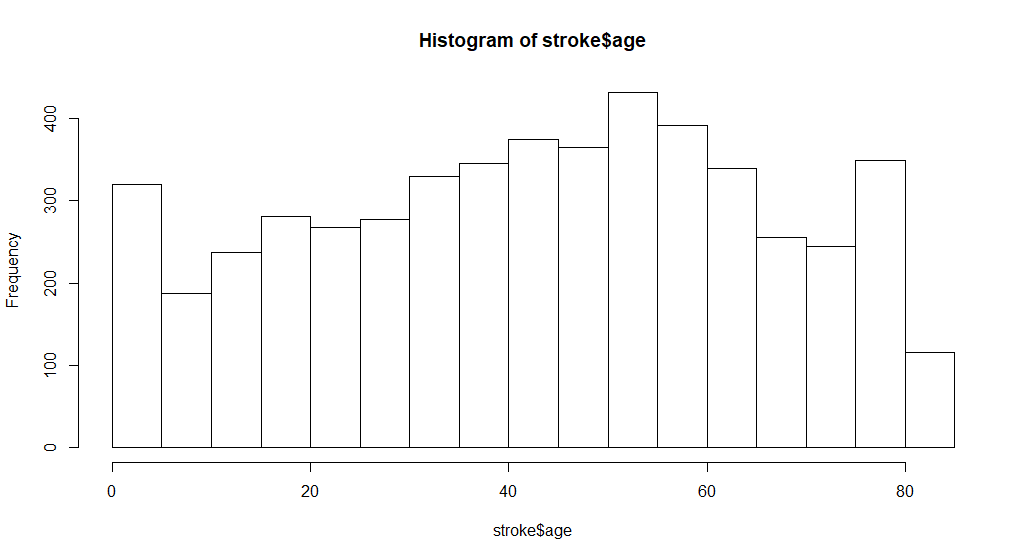
\includegraphics[scale=.5]{stroke-ages}
\end{enumerate}
\end{document}